\documentclass[
    12pt,
    a4paper,
    ngerman,
    color=3b,% Farbe für Hervorhebungen auf Basis der Deklarationen in den
    %type=intern,
    %titlepage=true,
    marginpar=false,
    colorback=false,
    %logo=head,
    leqno,
]{tudaexercise}
\usepackage{import}
% Import all Packages from Main Preamble with relative Path
\subimport*{../../}{preamble}
% Get Labels from Main Document using the xr-hyper Package
\externaldocument{../../AuD-Zusammenfassung-2020}
\externaldocument{../Kapitel_1/Kapitel_1}
\externaldocument{../Kapitel_2/Kapitel_2}
\externaldocument{../Kapitel_3/Kapitel_3}
% Set Graphics Path, so pictures load correctly
\graphicspath{{../../}}


\begin{document}
\section{Advanced Data Structures}\label{Advanced Data Structures}\index{Advanced Data Structures}
\subsection{Rot-Schwarz-Bäume}\label{Rot-Schwarz-Baeume}\index{Rot-Schwarz-Bäume}
    \begin{itemize}
        \item \fatsf{Definition}
            \begin{itemize}
                \item Binärer Suchbaum mit Zusatzeigenschaften
                \item Zusatzeigenschaften:
                    \begin{itemize}
                        \item Jeder Knoten hat die Farbe rot oder schwarz
                        \item Die Wurzel ist schwarz
                        \item Wenn ein Knoten rot ist, sind seine Kinder schwarz ("`Nicht-Rot-Rot-Regel"')
                        \item Für jeden Knoten hat jeder Pfad zu einem Blatt die selbe Anzahl an gleichen schwarzen Knoten
                    \end{itemize}
                \item Halbblätter im RBT sind schwarz
                \item Schwarzhöhe\index{Schwarzhöhe} eines Knoten: \\
                        Eindeutige Anzahl von schwarzen Knoten auf dem Weg zu einem Blatt im Teilbaum des Knoten
                \item Für leeren Baum gibt Schwarzhöhe = 0 ($SH(nil)=0$)
                \item Höhe eines Rot-Schwarz-Baums
                    \begin{itemize}
                        \item $h \leq 2 \cdot log_2(n+1)$  ($n$ Knoten)
                        \item In jedem Unterteilbaum gleiche Anzahl schwarzer Knoten
                        \item Maximal zusätzlich gleiche Anzahl roter Knoten auf diesem Pfad
                        \item Einigermaßen ausbalanciert $\Rightarrow$ Höhe $O(log~n)$
                    \end{itemize}
                \item Alle folgenden Algorithmen arbeiten mithilfe eines Sentinels (zeigt auf sich selbst)
            \end{itemize}
            \begin{figure}[ht]
                \centering
                \includestandalone[width=.5\textwidth]{pictures/baum_beispiel/baum_beispiel}% 
                \caption{Beispielhafte Darstellung wie in \ref{Definitionen fuer Datenstrukturen}}
                \label{fig:red_black_tree_example}
            \end{figure}
            \clearpage
        \item \fatsf{Einfügen}
            \begin{itemize}
                \item Laufzeit: $\Theta(h)$ ($h$ jedoch $log~n$)
                \item[1.] Finde Elternknoten wie im BST (\hyperref[BST-Insert]{BST-Einfüge Algorithmus})
                \item[2.] Knoten als Kind von Elternknoten anfügen
                \item[3.] Färbe den neuen Knoten rot
                \item[4.] Wiederherstellen der Rot-Schwarz-Bedingung\index{fixColorsAfterInsertion()}
                            \begin{ccode}[autogobble,escapeinside=||]{title={insert(T,z) //z.left==z.right==nil;}}
                                x=T.root; px=T.sent;
                                WHILE x != nil DO                   //Bis zum passenden Blatt gehen
                                    px=x;
                                    IF x.key > z.key THEN
                                        x=x.left;
                                    ELSE
                                        x=x.right;
                                z.parent=px;
                                IF px==T.sent THEN                  // Einfügen
                                    T.root=z
                                ELSE
                                    IF px.key > z.key THEN
                                        px.left=z;
                                    ELSE
                                        px.right=z;
                                z.color=red;                        // ab hier anders als bei BST-Insert
                                fixColorsAfterInsertion(T,z);
                            \end{ccode} 
                \item Hilfsmethode \texttt{rotateLeft}\index{rotateLeft()}
                            \begin{ccode}[autogobble]{title={rotateLeft(T,x)}}
                            y = x.right;
                            x.right = y.left;
                            IF y.left != nil THEN
                                y.left.parent = x;
                            y.parent = x.parent;
                            IF x.parent == T.sent THEN
                                T.root = y;
                            ELSE
                                IF x == x.parent.left THEN
                                    x.parent.left = y;
                                ELSE
                                    x.parent.right = y;
                            y.left = x;
                            x.parent = y;
                            \end{ccode}
            \end{itemize}
\clearpage
        \item \fatsf{fixColorsAfterInsertion}
        \begin{itemize}
            \item Beim Aufrufen werden zwei Bedingungen potentiell verletzt: 
            \begin{itemize}
                \item[1.] root ist nicht mehr schwarz
                \item[2.] wenn eine Node rot ist müssen beide Kinder schwarz sein
            \end{itemize}
            \item Also müssen wir:
            \begin{itemize}
                \item nach rotation die root des aktuellen Teilbaumes auf schwarz setzen
                \item Überprüfen, ob RSB-Bedingung verletzt wurde
                \item Bloß wenn das parent auch rot ist kommen wir in Verlegenheit $\Longrightarrow$ wir müssen den Algorithmus starten
            \end{itemize} 
            
            \begin{minipage}{.5\textwidth}
            \item Fälle falls Parent rot ist:
            \begin{itemize}
                \item[1.] Onkel ist ebenfalls rot $\Rightarrow$ parent und Onkel werden schwarz gefärbt und Grandparent wird rot gefärbt
                \item[2.] Onkel ist schwarz und z hat andere Kindrichtung wie z.p $\Rightarrow$ zu Fall 3 durch rotation konvertieren
                \item[3.] Onkel ist schwarz und z hat gleiche Kindrichtung wie z.p $\Rightarrow$ z.p wird schwarz, z.p.p wird rot, und es wird um z.p.p entgegen der Kindrichtung gedreht
            \end{itemize}
            \end{minipage}
            \begin{minipage}{.4\textwidth}
                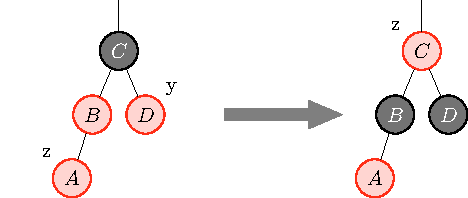
\includegraphics[width=\textwidth]{pictures/fixColorsAfterInsertionCases/case 1}
                \captionof*{figure}{Fall 1}
            \end{minipage}\\
        \end{itemize}
        \begin{ccode}[autogobble,fontsize=\small]{title={fixColorsAfterInsertion(T,z)}}
            WHILE z.parent.color == red DO                  // solange der Elternknoten rot ist
                IF z.parent == z.parent.parent.left THEN    // Linkes Kind (if-Fall)
                    y = z.parent.parent.right;
                    IF y != nil AND y.color == red THEN     // Fall 1
                        z.parent.color = black;
                        y.color = black;
                        z.parent.parent.color = red;
                        z = z.parent.parent;                // rekursiv nach oben weiterführen
                    ELSE                                    // Fall 2
                        IF z == z.parent.right THEN         // Zwischenfall (2.1)
                            z = z.parent;
                            rotateLeft(T,z);
                        z.parent.color = black;
                        z.parent.parent.color = red;
                        rotateRight(T, z.parent.parent);
                ELSE                                        // Rechtes Kind (else-Fall)
                    // Tauschen von rechts und links
                T.root.color = black;                       // Setzen der Wurzel auf Schwarz
            \end{ccode}
            \begin{minipage}{.5\textwidth}
                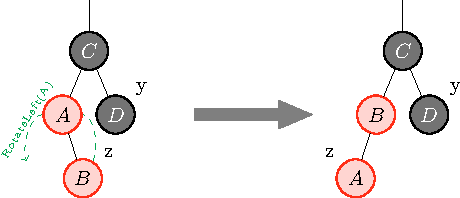
\includegraphics{pictures/fixColorsAfterInsertionCases/case2}
                \captionof*{figure}{Fall 2}
            \end{minipage}
            \begin{minipage}{.4\textwidth}
            \nopagebreak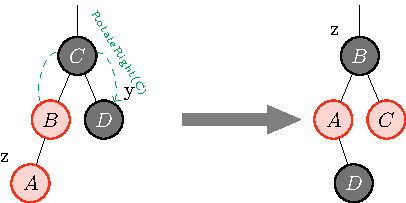
\includegraphics{pictures/fixColorsAfterInsertionCases/case3}
                \captionof*{figure}{Fall 3}
            \end{minipage}
            \clearpage
        \item \fatsf{Löschen}
            \begin{itemize}
                \item Laufzeit: $O(h) = O(log~n)$
                \item analog zum binären Suchbaum, aber neue Node erbt Farbe der alten Node
                \item Wenn "`neue"' Node schwarz war $\Rightarrow$ Fixup
                \item Verschiedene Fälle, die auch gegenseitig Voraussetzungen füreinander sind 
                \item Da das Ganze jedoch etwas umfangreicher ist, findet es sich nicht hier in der Zusammenfassung
            \end{itemize}
        
        \item \fatsf{Worst-Case-Laufzeiten}
            \begin{itemize}
                \item {\makebox[2cm][l]{Einfügen: }} $\Theta(log~n)$
                \item {\makebox[2cm][l]{Löschen: }} $\Theta(log~n)$
                \item {\makebox[2cm][l]{Suchen: }} $\Theta(log~n)$
            \end{itemize}
    \end{itemize}
    \subsection{AVL-Bäume}\label{AVL-Baeume}\index{AVL-Bäume}
    \begin{itemize}
        \item \fatsf{Definition:}
            \begin{itemize}
                \item $h \leq 1.441 \cdot log~n$ (optimierte Konstanten - 1,441 vs 2 (RBT))
                \item Binärer Suchbaum
                \item Allerdings Balance in jedem Knoten nur $-1,0,1$
                \item Balance für $x$: $B(x)$ = Höhe(rechter Teilbaum) - Höhe(linker Teilbaum)
                \item[]\index{linkslastig}\index{rechtslastig}\index{balanciert} 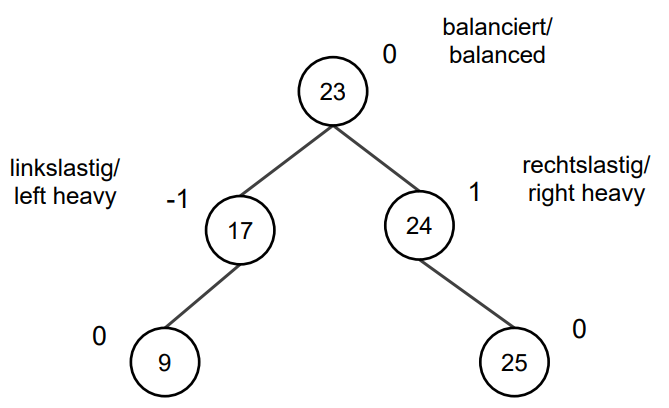
\includegraphics[width=7cm]{pictures/avlbaum.PNG}
            \end{itemize}
        
        \item \fatsf{AVL vs. Rot-Schwarz}
            \begin{itemize}
                \item \textit{AVL:}
                    \begin{itemize}
                        \item Einfügen und Löschen verletzen in der Regel öfter die Baum-Bedingung
                        \item Aufwendiger zum Rebalancieren
                    \end{itemize}
                \item \textit{Rot-Schwarz:}
                    \begin{itemize}
                        \item Suchen dauert evtl. länger
                    \end{itemize}
                \item \textit{Konklusion:}
                    \begin{itemize}
                        \item AVL geeigneter, wenn mehr Such-Operationen und weniger Einfügen und Löschen
                    \end{itemize}
                \item Gemeinsamkeiten:
                    \item AVL $\subset$ Rot-Schwarz
                    \item AVL Baum $\Rightarrow$ Rot-Schwarz-Baum mit Höhe $\left \lceil \frac{h+1}{2} \right \rceil$
                    \item Für jede Höhe $h \geq 3$ gibt es einen RBT, der kein AVL-Baum ist (AVL $\neq$ RBT)
            \end{itemize}
\clearpage
        \item \fatsf{Einfügen}
            \begin{itemize}
                \item Einfügen funktioniert wie beim Binary Search Tree mit Sentinel\index{Sentinel}
                \item Erfordert danach jedoch Rebalancieren weiter oben im Baum
                \item Rebalancieren: (verschiedene Fälle)
                \item[]
                    \begin{minipage}{0.45\textwidth}
                        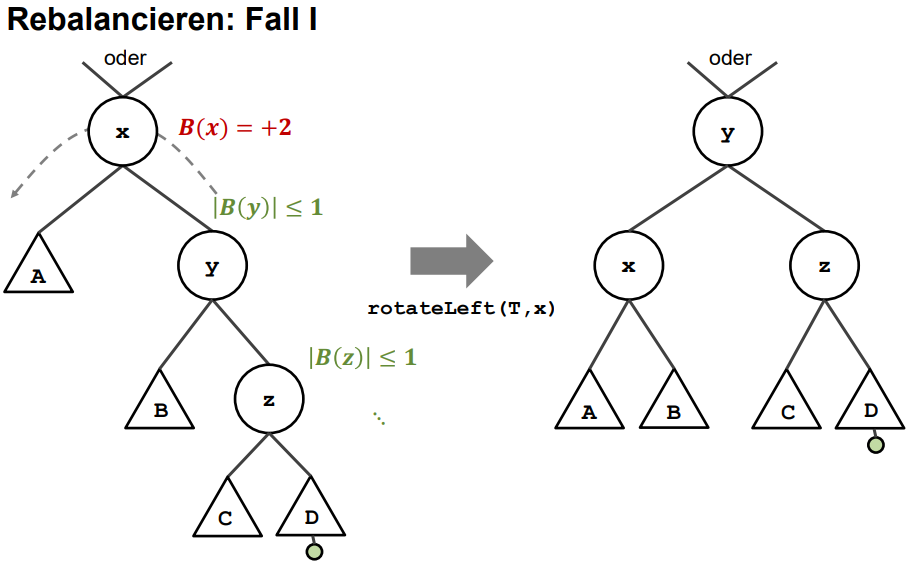
\includegraphics[width=7cm]{pictures/avlcase1.PNG}
                    \end{minipage}
                    \begin{minipage}{0.45\textwidth}
                        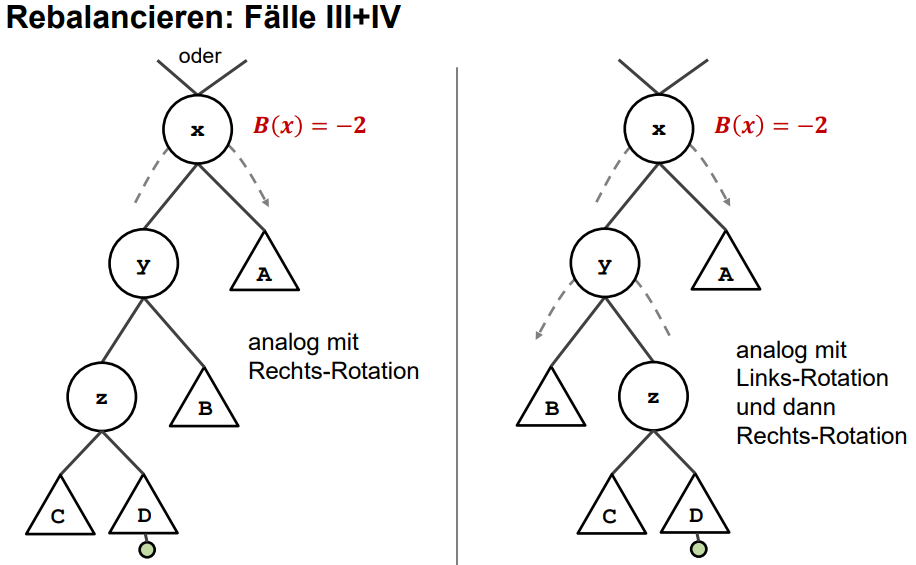
\includegraphics[width=7cm]{pictures/avlcase34.PNG} 
                    \end{minipage}
                \item[]
                    \begin{minipage}{0.45\textwidth}
                        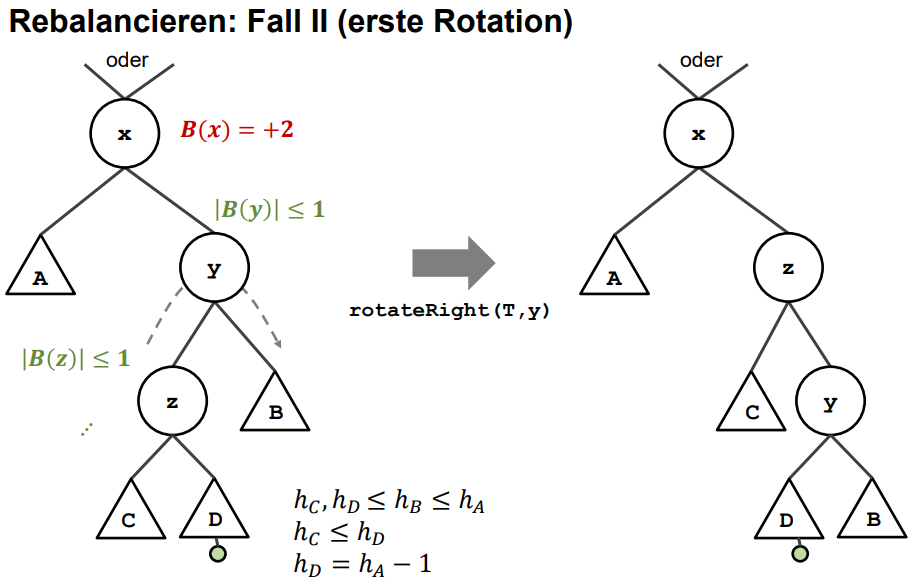
\includegraphics[width=7cm]{pictures/avlcase2_1.PNG}
                    \end{minipage}
                    \begin{minipage}{0.45\textwidth}
                        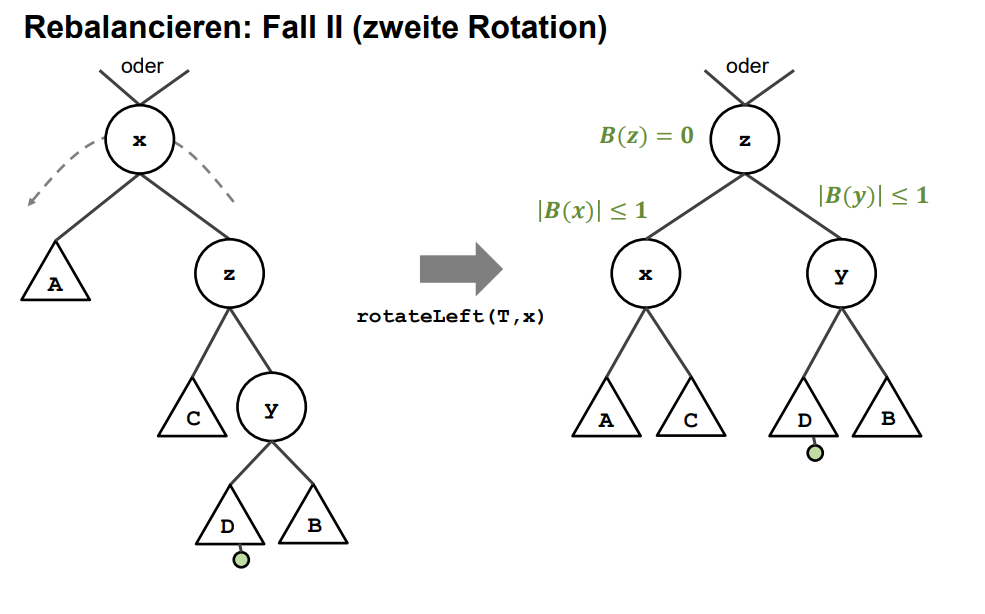
\includegraphics[width=7cm]{pictures/avlcase2_2.PNG}
                    \end{minipage}
            \end{itemize}

        \item \fatsf{Löschen}
            \begin{itemize}
                \item Analog zum binären Suchbaum
                \item Rebalancieren bis eventuell in die Wurzel notwendig
            \end{itemize}

        \item \fatsf{Worst-Case-Laufzeiten}
            \begin{itemize}
                \item {\makebox[2cm][l]{Einfügen: }} $\Theta(log~n)$
                \item {\makebox[2cm][l]{Löschen: }} $\Theta(log~n)$
                \item {\makebox[2cm][l]{Suchen: }} $\Theta(log~n)$
                \item theoretisch bessere Konstanten als RBT
                \item in Praxis aber nur unwesentlich schneller
            \end{itemize}
    \end{itemize}
    \clearpage
    \subsection{Splay-Bäume}\label{Splay-Baeume}\index{Splay-Bäume}
    \begin{itemize}
        \item \fatsf{Definition}
            \begin{itemize}
                \item selbst-organisierende Listen
                \item Ansatz: Einmal angefragte Werte werdeb wahrs. noch öfter angefragt
                \item Angefragte Werte nach oben schieben
                \item Splay-Bäume sind Untermenge von BST
            \end{itemize}
        
        \item \fatsf{Splay-Operationen}
            \begin{itemize}
                \item Suchen oder Einfügen: Spüle gesuchten oder neu eingefügten Knoten an die Wurzel
                \item Splay:\index{splay} (Folge von Zig-,Zig-Zig-, Zig-Zag-Operationen)
                \item []
                    \begin{ccode}[autogobble]{title={splay(T,z)}}
                    WHILE z != T.root DO
                        IF z.parent.parent == nil THEN
                            zig(T,z);
                        ELSE
                            IF z == z.parent.parent.left.left OR
                               z == z.parent.parent.right.right THEN
                               zigZig(T,z);
                            ELSE
                                zigZag(T,z);
                    \end{ccode}
                \item[]
                \item[]\index{Zig-Zag} 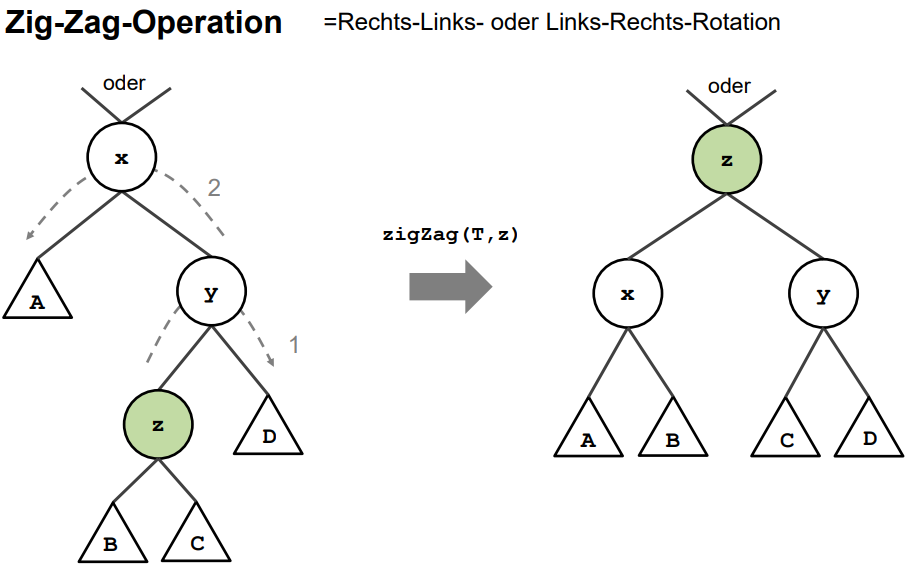
\includegraphics[width=12cm]{pictures/zigzag.PNG}
                \item[]\index{Zig-Zig} 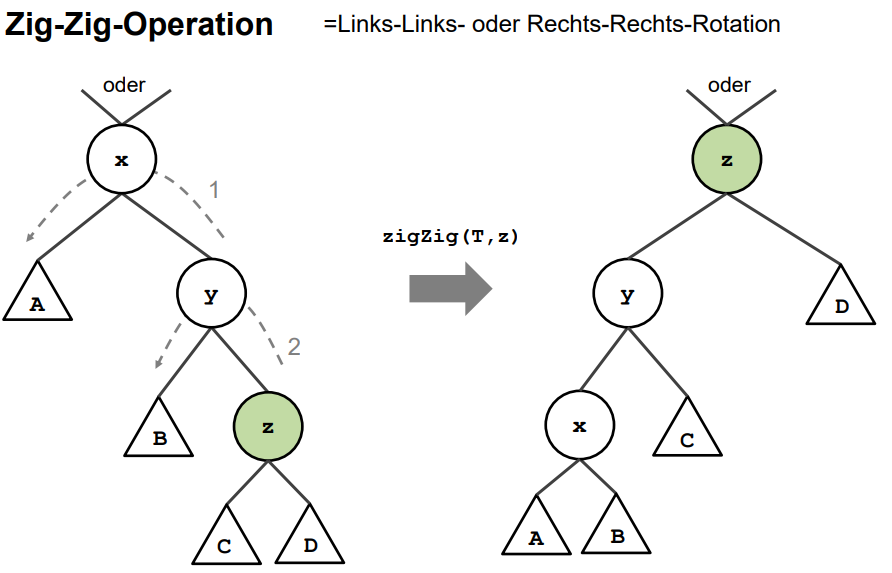
\includegraphics[width=11cm]{pictures/zigzig.PNG}
                \item[]\index{Zig} 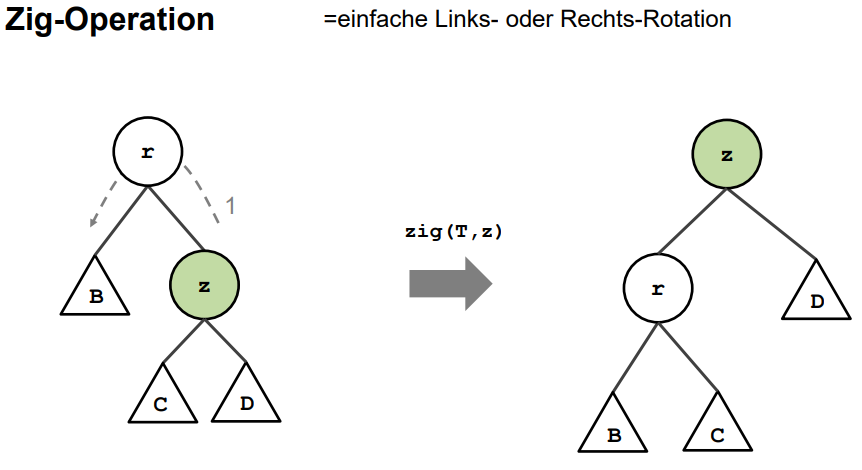
\includegraphics[width=11cm]{pictures/zig.PNG}
            \end{itemize}
        \vspace*{-1cm}
        \item \fatsf{Suchen}
            \begin{itemize}
                \item Laufzeit: $O(h)$
                \item Suche des Knotens wie im BST
                \item Hochspülen des gefundenen Knotens (alternativ zuletzt besuchter Knoten, falls nicht gefunden)
            \end{itemize}

        \item \fatsf{Einfügen}
            \begin{itemize}
                \item Laufzeit: $O(h)$
                \item Suche der Position wie im BST
                \item Einfügen und danach hochspülen des eingefügten Knotens
            \end{itemize}    

        \item \fatsf{Löschen}
            \begin{itemize}
                \item Laufzeit: $O(h)$
                \item[1.] Spüle gesuchten Knoten per Splay-Operation nach oben
                \item[2.] Lösche den gesuchten Knoten (Wenn einer der beiden entstehenden Teilbäume leer, dann fertig)
                \item[3.] Spüle den größten Knoten im linken Teilbaum nach oben (kann kein rechtes Kind haben)
                \item[4.] Hänge rechten Teilbaum an größten Knoten aus 3. an   
            \end{itemize}
        
        \item \fatsf{Laufzeit Splay-Bäume}
            \begin{itemize}
                \item Amortisierte Laufzeit: Laufzeit pro Operation über mehrere Operationen hinweg
                \item Worst-Case-Laufzeit pro Operation: $O(log_n~n)$
            \end{itemize}
    \end{itemize}
    \clearpage
    \subsection{Binäre Max-Heaps}\label{Binaere Max-Heaps}\index{Binäre Max-Heaps}
    \begin{itemize}
        \item \fatsf{Definition}
            \begin{itemize}
                \item Heaps sind keine BSTs
                \item Eigenschaften binäre Max-Heaps:
                    \begin{itemize}
                        \item bis auf das unterste Level vollständig und dort von links gefüllt ist
                        \item Für alle Knoten gilt: \texttt{x.parent.key $\geq$ x.key}
                        \item Maximum des Heaps steht damit in der Wurzel
                    \end{itemize}
                \item $h \leq log~n$, da Baum fast vollständig
            \end{itemize}

        \item \fatsf{Heaps durch Arrays}
            \begin{itemize}
                \item[] 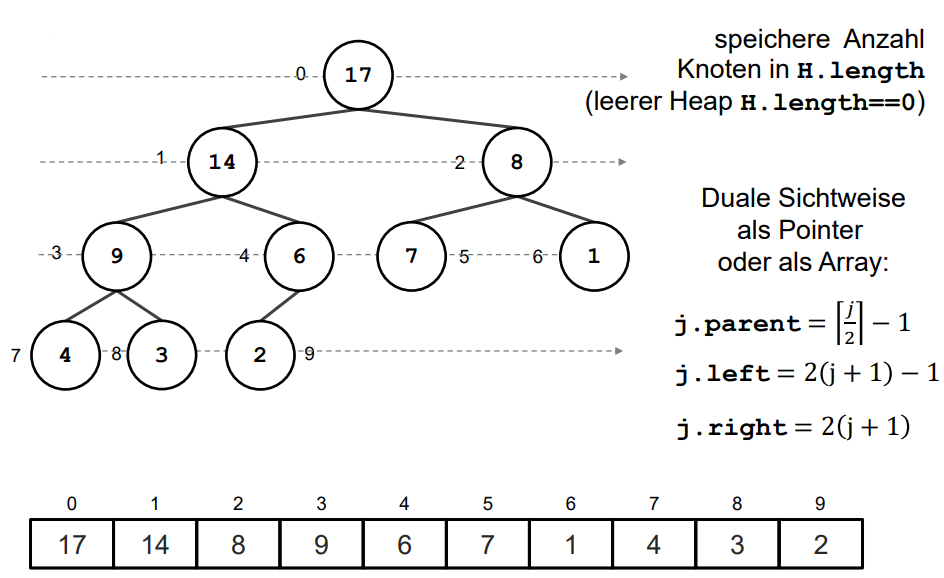
\includegraphics[width=8cm]{pictures/heapArr.PNG}
            \end{itemize}

        \item \fatsf{Einfügen}
            \begin{itemize}
                \item Idee: Einfügen und danach Vertauschen nach oben, bis Max-Eigenschaft wieder erfüllt ist
                \item Laufzeit: $O(h) = O(log~n)$
                \item[]
                    \begin{ccode}[autogobble]{title={insert(H,k) // als unbeschränktes Array}}
                    H.length = H.length + 1;
                    H.A[H.length-1] = k;

                    i = H.length - 1;
                    WHILE i > 0 AND H.A[i] > H.A[i.parent]
                        SWAP(H.A, i, i.parent);
                        i = i.parent;
                    \end{ccode}
            \end{itemize}
\clearpage
        \item \fatsf{Lösche Maximum}
            \begin{itemize}
                \item[1.] Ersetze Maximum durch "`letztes"' Blatt
                \item[2.] Vertausche Knoten durch Maximum der beiden Kinder (\texttt{heapify})
                \item[]\index{extract-max(H)}\index{heapify(H,i)}
                    \begin{minipage}{0.33\textwidth}
                        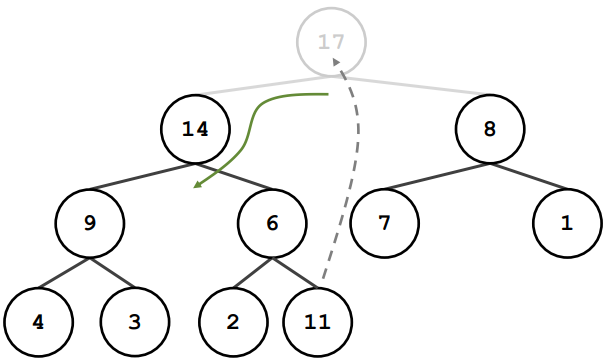
\includegraphics[width=6cm]{pictures/heapDelete.PNG}
                    \end{minipage} 
                    \begin{minipage}{0.57\textwidth}
                        \begin{ccode}[autogobble]{title={extract-max(H)}}
                        IF isEmpty(H) THEN return error "underflow";
                        ELSE
                            max = H.A[0];
                            H.A[0] = H.A[H.length - 1];
                            H.length = H.length - 1;
                            heapify(H, 0);
                            return max;
                        \end{ccode}
                    \end{minipage}
                \item[]
                    \begin{ccode}[autogobble]{title={heapify(H, i)}}
                    maxind = i;
                    IF i.left < H.length AND H.A[i]<H.A[i.left] THEN
                        maxind = i.left;
                    IF i.right < H.length AND H.A[maxind]<H.A[i.right] THEN
                        maxind = i.right;

                    IF maxind != i THEN
                        SWAP(H.A, i, maxind);
                        heapify(H, maxind);
                    \end{ccode}
            \end{itemize}

        \item \fatsf{Heap-Konstruktion aus Array}
            \begin{itemize}
                \item Blätter sind für sich triviale Max-Heaps
                \item Bauen von Max-Heaps für Teilbäume mithilfe Rekursion per \texttt{heapify} 
                \item (Array nicht unbedingt in richtiger Reihenfolge)
                \item[]\index{buildHeap(H,A)}\index{HeapSort(H,A)}
                    \begin{ccode}[autogobble]{title={buildHeap(H.A) // Array in H.A}}
                    H.length = A.length;
                    FOR i = ceil((H.length-1)/2) - 1 DOWNTO 0 DO
                        heapify(H.A,i);
                    \end{ccode}
            \end{itemize}

        \item \fatsf{Heap-Sort}
            \begin{itemize}
                \item Idee: Bauen des Heaps aus Array und dann Extraktion des Maximums
                \item[]
                    \begin{ccode}[autogobble]{title={heapSort(H.A)}}
                    buildHeap(H.A)                  // Bauen des Heaps
                    WHILE !isEmpty(H) DO
                        PRINT extract-max(H);       // Ausgabe des Maximums bis Heap leer ist
                    \end{ccode}
            \end{itemize}
    \end{itemize}
    \clearpage
    \subsection{B-Bäume}\label{B-Baeume}\index{B-Baeume}
    \begin{itemize}
        \item \fatsf{Definition}
            \begin{itemize}
                \item Jeder B-Baum hat einen angebenen Grad also z.B. $t=2$
                \item Eigenschaften:
                    \begin{itemize}
                        \item Wurzel zwischen $[1,...,2t-1]$ Werte
                        \item Knoten zwischen $[t-1,...2t-1]$ Werte
                        \item Werte innerhalb eines Knotens aufsteigend geordnet
                        \item Blätter haben alle die gleiche Höhe
                        \item Jeder innere Knoten mit $n$ Werten hat $n+1$ Kinder, sodass gilt:
                        \item[] $k_0 \leq key[0] \leq k_1 \leq key[1] \leq ... \leq k_{n-1} \leq key[n-1] \leq k_n$
                    \end{itemize}
                \item[] 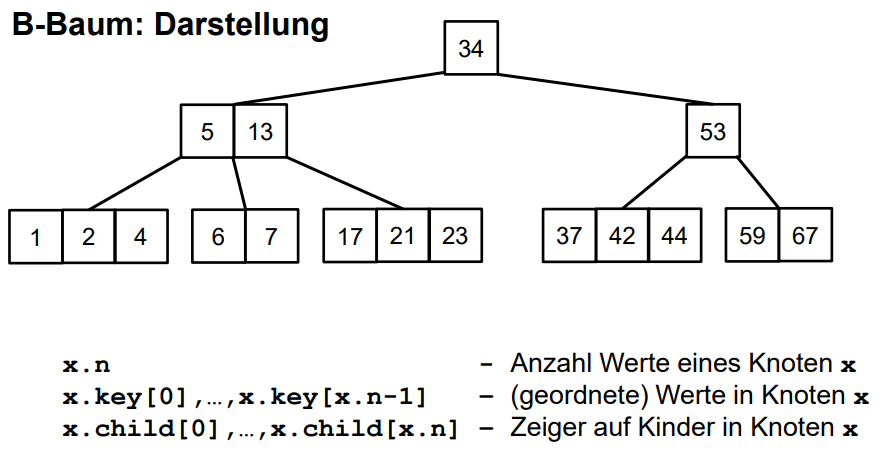
\includegraphics[width=15cm]{pictures/bbaum.PNG}
                \item Höhe B-Baum: $h \leq log_t \frac{n+1}{2}$ (Grad $t$ und $n$ Werte)
                \item B-Baum wird für größere $t$ flacher
            \end{itemize}
        \clearpage
        \item \fatsf{Suche}
            \begin{itemize}
                \item[] 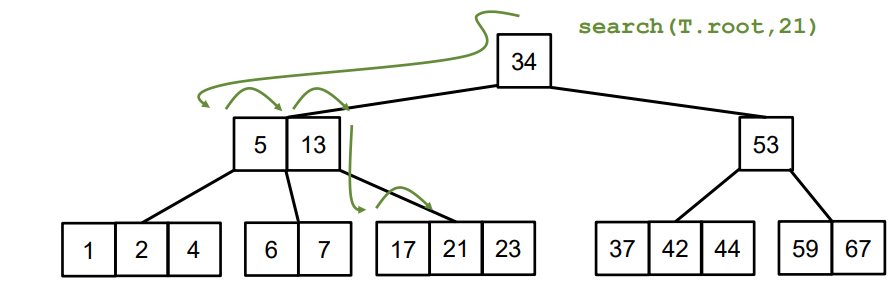
\includegraphics[width=12cm]{pictures/bbaumSuche.PNG}
                \item[]
                    \begin{ccode}[autogobble]{title={search(x, k)}}
                    WHILE x != nil DO
                        i = 0;
                        WHILE i < x.n AND x.key[i] < k DO
                            i++;
                        IF i < x.n AND x.key[i] == k THEN
                            return(x, i);
                        ELSE
                            x = x.child[i];
                    return nil;
                    \end{ccode}
            \end{itemize}


        \item \fatsf{Einfügen}
            \begin{itemize}
                \item Einfügen erfolgt immer in einem Blatt
                \item Falls das Blatt voll ist, muss jedoch gesplittet werden
                \item $\Rightarrow$ Beim Durchlaufen des Baumes an jeder notwendigen (voll) Position splitten
                \item Splitten:\index{Splitten}
                    \begin{itemize}
                        \item Bricht volle Node auf und fügt mittleren Wert zur Elternnode hinzu
                        \item Aus den anderen Werten entstehen nun jeweils eigene Kinder
                        \item An der Wurzel splitten erzeugt neue Wurzel und erhöht Baumhöhe um eins
                    \end{itemize}
                \item Ablauf zusammengefasst:
                    \begin{enumerate}
                        \item Start bei Wurzel, falls kein Platz mehr splitten
                        \item Durchlaufen des Baumes bis zur richtigen Position und immer, falls voll, splitten
                        \item Einfügen der Node (fertig)
                    \end{enumerate}
                \item[]
                    \begin{ccode}[autogobble]{title={insert(T, z)}}
                    Wenn Wurzel schon 2t-1 Werte, dann splitte Wurzel
                    Suche rekursiv Einfügeposition:
                        Wenn zu besuchendes Kind 2t-1 Werte, splitte es erst
                    Füge z in Blatt ein
                    \end{ccode}
            \end{itemize}

\clearpage

        \item \fatsf{Löschen}
            \begin{itemize}
                \item Wenn Blatt noch mehr als t-1 Werte, kann der Wert einfach entfernt werden
                \item Allerdings durchlaufen wir hier den Baum auch wieder von oben und stellen gewisse Voraussetzungen her
                \item Durchlaufen des Baumes von oben und Anwendung der folgenden Algorithmen
                \item[]
                    \begin{minipage}{0.25\textwidth}
                        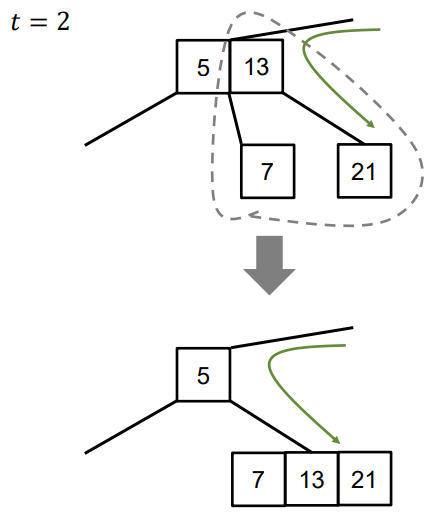
\includegraphics[width=4cm]{pictures/bbaumMelt.PNG}
                    \end{minipage}
                    \begin{minipage}{0.65\textwidth}
                        Allgemeines Verschmelzen:\index{Verschmelzen}
                        \begin{itemize}
                            \item Kind und alle rechten/linken Geschwisterknoten nur $t-1$ Werte
                            \item Wenn Elternknoten vorher min. $t$ Werte
                            \item[] $\Rightarrow$ keine Änderung oberhalb notwendig
                        \end{itemize}
                    \end{minipage}
                \item[]
                    \begin{minipage}{0.25\textwidth}
                        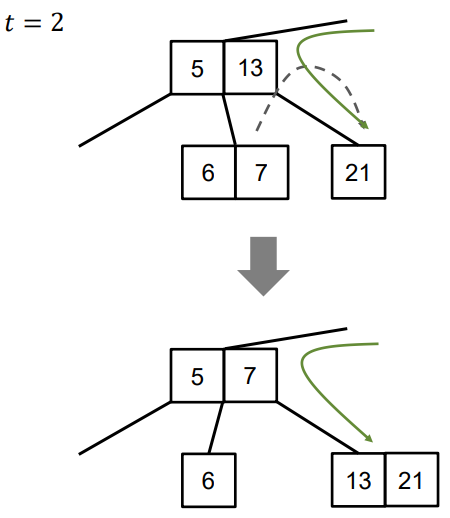
\includegraphics[width=4cm]{pictures/bbaumRot.PNG}
                    \end{minipage}
                    \begin{minipage}{0.65\textwidth}
                        Allgemeines Rotieren/Verschieben:
                        \begin{itemize}
                            \item Kind nur $t-1$ Werte
                            \item Geschwister jedoch mehr als $t-1$ Werte
                            \item keine Änderung oberhalb notwendig
                        \end{itemize}
                    \end{minipage}
                    
                    \item Code:
                \item[]
                    \begin{ccode}[autogobble]{title={delete(T, k)}}
                    Wenn Wurzel nur 1 Wert und beide Kinder t-1 Werte, 
                    verschmelze Wurzel und Kinder (reduziert Höhe um 1)
                    Suche rekursiv Löschposition:
                        Wenn zu besuchendes Kind nur t-1 Werte, 
                        verschmelze es oder rotiere/verschiebe
                    Entferne Wert k im inneren Knoten/Blatt             
                    // Ohne Probleme, aufgrund vorheriger Anpassung
                    \end{ccode}
            \end{itemize}

        \item \fatsf{Laufzeiten}
            \begin{itemize}
                \item {\makebox[2cm][l]{Einfügen: }} $\Theta(log_t~n)$
                \item {\makebox[2cm][l]{Löschen: }} $\Theta(log_t~n)$
                \item {\makebox[2cm][l]{Suchen: }} $\Theta(log_t~n)$
                \item Nur vorteilhaft wenn Daten blockweise eingelesen werden
                \item $\mathcal{O}$-Notation versteckt hier konstanten Faktor $t$ für Suche innerhalb eines Knotens
            \end{itemize}
    \end{itemize}
    \clearpage
\end{document}
